\begin{center}
	\section{PROBLEMA DE INVESTIGACIÓN}
\end{center}

%%\begin{center}
%%	\begin{figure}[hb!]
%%		\subfigure[Una rana]{
%%			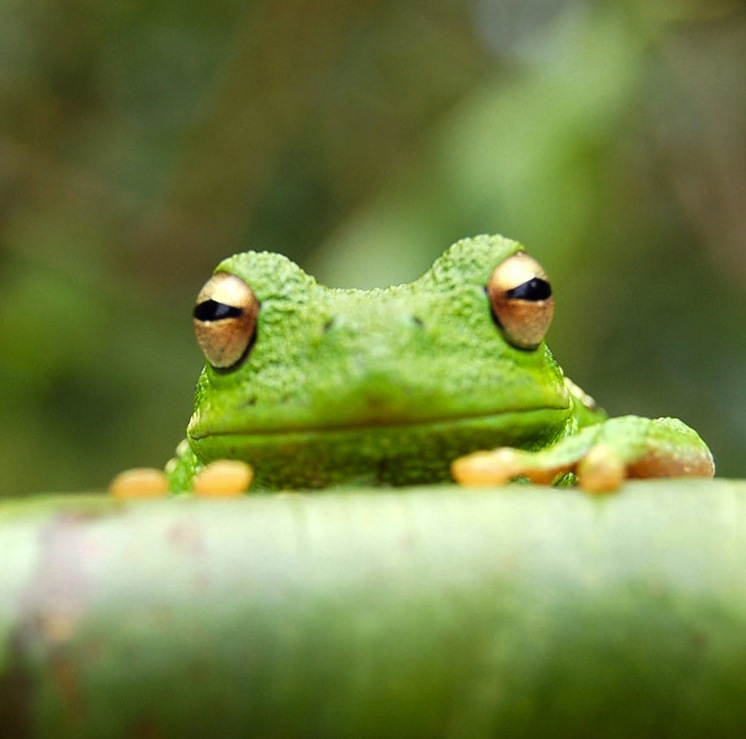
\includegraphics[scale=.2]{frog.jpg} \label{fig:frog}
%%		}
%%		\subfigure[Otra rana (o acaso es la misma?)]{
%%			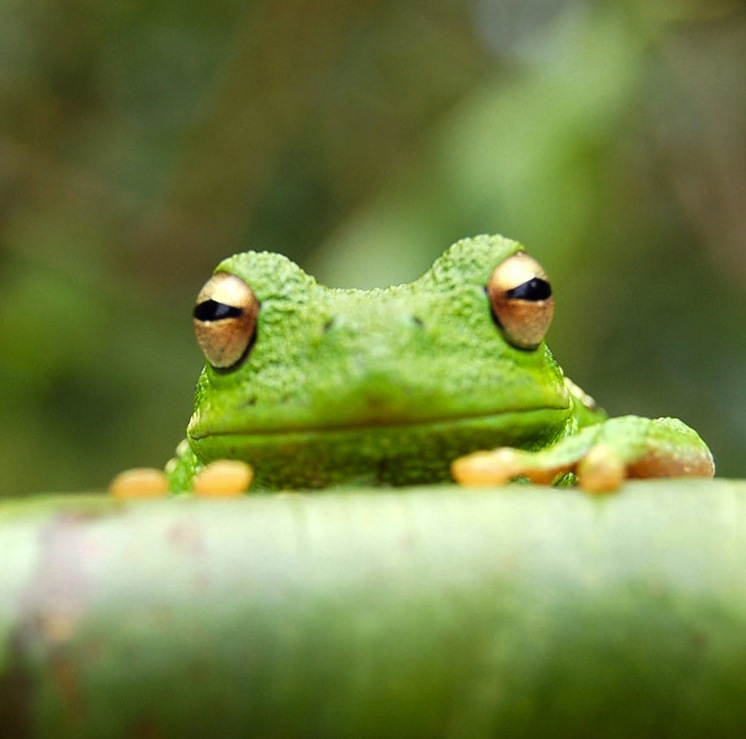
\includegraphics[scale=.2]{frog.jpg} \label{fig:anotherfrog}
%%		}
%%		\caption[Unas ranas]{La rana de la izquierda a primera vista parece ser la misma rana de la derecha.}
%%		\label{fig:fig1}
%%	\end{figure}
%%\end{center}

En los años sesenta (60) los Algoritmos Gen\'eticos (AGs) se conocían como \textit{planes reproductivos}; no obstante fue el científico Holland (\cite{Holland1975}) quien promovió la idea de ``\textit{algoritmos genéticos}", partiendo como base de que todo ocurre por las interacciones locales entre individuos, y entre estos lo que les rodea.  Unos años más tarde  (\cite{Holland1992}) divulga que los programas que ``evolucionan", simulando en cierto grado la selección natural, alcanzan a resolver problemas complejos que ni siquiera quienes los crearon comprenden plenamente; haciendo de esta manera obtener resultados sorprendentes que en ningún momento fueron imaginados y/o deliberados.\\

Los AGs son m\'etodos adaptativos, utilizados en la mayor\'ia de los casos para resolver problemas de b\'usqueda y optimizaci\'on de par\'ametros,  inspirados en la reproducci\'on sexual y en el principio de supervivencia del m\'as apto (\cite{Fogel2000}) (\cite{Fogel2006}). En un contexto m\'as alineado y proporcionado por Goldberg alude que ``\textit{los Algoritmos Gen\'eticos son algoritmos de b\'usqueda basados en la mec\'anica de selecci\'on natural y de la gen\'etica natural. Combinan la supervivencia del m\'as apto entre estructuras de secuencias con un intercambio de informaci\'on estructurado, aunque aleatorizado, para constituir as\'i un algoritmo de b\'usqueda que tenga algo de las genialidades de las b\'usquedas humanas}" (\cite{Goldberg1989}). Lo anterior determina que los genes de los especímenes mejor adaptados se propagarán en sucesivas generaciones hacia un número de especímenes creciente; consiguiendo de esta forma producir descendientes con caracteristicas cada vez mejores y adaptables.\\

En el año 2008 a nivel mundial ya existían diferentes implementaciones de algoritmos genéticos en sistemas de inteligencia artificial; pero algo que tomó fuerza y se convirtió en una técnica de desarrollo comúnmente utilizada fue la ingeniería de software basada en componentes; aplicado para el desarrollo de grandes sistemas empresariales como también en aplicaciones para entornos incrustados (\cite{Adamek2008}). En ese entonces, no se percibía el impacto que traería consigo la aplicación de la ingeniería de software con este enfoque en los sistemas de información; y más aún que se lograra desarrollar software basado en componentes para algoritmos genéticos, hasta que en el año 2013 es liberada la primera versión de Goldenberry (\cite{Rojas-Galeano2013}) (\cite{NestorTesis2013}); una caja de herramientas \textit{open source} con componentes visuales de Estimación de Algoritmos de Distribución (EDA) para la optimización basada en búsqueda estocástica.  El objetivo principal de esta versión de Goldenberry era proporcionar un banco de trabajo fácil de usar para investigadores y profesionales, basado en la versatilidad de la programación visual de \textit{Orange} y de los poderosos principios de reutilización y pegamento del desarrollo de software basado en componentes.\\   

Más tarde un grupo de investigadores de la Universidad Distrital Franciso José de Caldas (\cite{LeidyTowars}), comezaron a cuestionarse si sería factible y ventajoso una arquitectura de software basada en componentes para algoritmos evolutivos; utilizando la misma plataforma de programación visual basada en componentes.  No obstante, en el año 2015 (\cite{LeidyVisual}) el equipo de investigadores construyeron y lanzaron una nueva librería para la programación de algoritmos de computación evolutiva (CE) llamada \textit{Goldenberry 2.0}, bajo el enfoque de construcción de sistemas mediante componentes, utilizando módulos de software prefabricados, fácil de ensamblar y que se puedan realizar en un ambiente visual amigable con el usuario como lo es \textit{Orange}.\\

\subsection{PLANTEAMIENTO  DEL PROBLEMA}

Actualmente han salido al mercado dos versiones de Goldenberry (1.0 (\cite{Rojas-Galeano2013}) y 2.0 (\cite{LeidyVisual})); en donde la orientación ha sido complementar la colección de componentes de software desarrollados, sin embargo; en la versión 1.0 se ha identificado que la deficiencia más significativa ha sido no haberse aplicado un proceso riguroso de ingeniería de software basado en componentes, ya que el nivel de especificación de cada componente fue de manera sutil. Mientras que en la versión 2.0 a pesar de contemplar este tipo de enfoque, su falencia radica en la usuabilidad de la librería en el ambiente de programación visual \textit{Orange}; ya que este es un programa libre y de terceros, el cual se actualiza constantemente, haciendo que los componentes de software desarrollados en Goldenberry 2.0 no puedan ser compilados, ejecutados y utilizados en la última versión de \textit{Orange 3.4}.\\

En ese orden de ideas, se hace necesario desarrollar una alternativa de solución que permita integrar las versiones anteriores de Goldenberry; pero que a su vez esta pueda funcionar correctamente en \textit{Orange 3.4}.  Por otro lado, se requiere añadir una extensión a Goldenberry con un componente de software de computación evolutiva que permita ampliar la gama de colecciones de componentes de software para algoritmos genéticos.\\           

\subsection{FORMULACIÓN DEL PROBLEMA}
%\lipsum[4-8] \index{Fomulación}
De acuerdo a lo expuesto anteriormente, se formula la siguiente pregunta de investigación:

\subsubsection{Pregunta de investigación}
%\lipsum[4-8] \index{Pregunta}
¿Cómo contribuir al funcionamiento, portabilidad y usabilidad de la librería Goldenberry en la plataforma de progamación visual \textit{Orange}?

\subsection{SISTEMATIZACIÓN DEL PROBLEMA}
\begin{itemize}
	\item ¿Cómo es el funcionamiento de las versiones anteriores de la plataforma Goldenberry?
	\item ¿Qué se necesita para lograr el funcionamiento de Goldenberry en la la última versión de \textit{Orange 3.4}? 
	\item ¿Cómo lograr realizar un proceso detallado de pruebas que garantice el óptimo funciomiento del nuevo componente de software a desarrollar?   
	\item ¿Cuáles serán los pasos necesarios para considerar que Goldenberry 3.0 sea un complemento ``\textit{add-on}" en el estandar de distribución de \textit{Orange}?
\end{itemize}